\subsection{Mean Value Theorem (MVT)}\label{subsec:mean-value-theoremnullmvtnull}

Given that $f(x)$ is continuous $\forall x \in [a,b]$ and differentiable
$\forall x \in (a,b)$, $\exists c \in (a,b)$ such that $f'(c)=\frac{f(b)-f(a)}{b-a}$.

\bigskip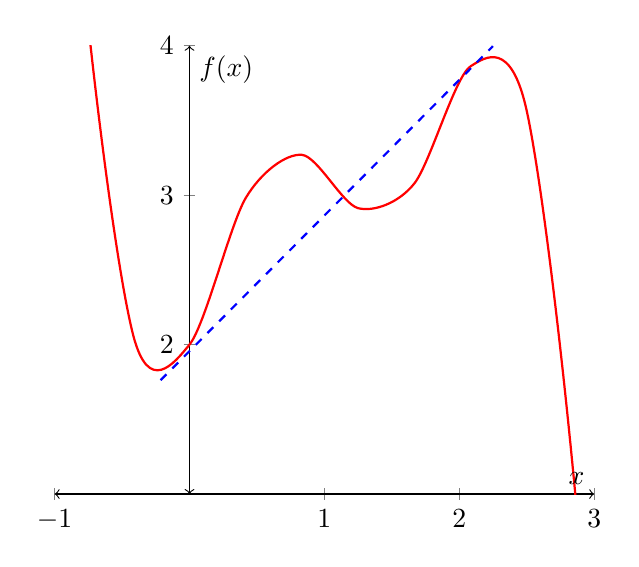
\begin{tikzpicture}
    \begin{axis}[
        xmin=-1,xmax=3,
        ymin=1,ymax=4,
        axis x line=middle,
        axis y line=middle,
        axis line style=<->,
        xlabel={$x$},
        ylabel={$f(x)$}
        ]
    \addplot[red,thick,smooth] {sin(3*deg(x))-x^3+3*x^2-x+2};
    \draw [dashed, thick, blue] (-.214,1.762) -- (2.249,3.997);
    \end{axis}
\end{tikzpicture}

\subsection{Intermediate Value Theorem (IVT)}\label{subsec:intermediate-value-theoremnullivtnull}

Let $f(x)$ be continuous $\forall x \in [a,b]$. Let $m$ between $f(a)$ and $f(b)$.
$\exists c \in (a,b)$ such that $f(c)=m$.

\bigskip\begin{tikzpicture}
    \begin{axis}[
        xmin=0,xmax=4,
        ymin=0,ymax=4,
        axis x line=middle,
        axis y line=middle,
        axis line style=<->,
        xlabel={$x$},
        ylabel={$f(x)$}
        ]
    \addplot[red,thick,smooth,domain=0:1] {x^2};
    \addplot[blue,thick,smooth,domain=1:1.5,dashed] {x^2};
    \addplot[red,thick,smooth,domain=1.5:5] {x^2};
    \node[label={180:{$a$}}] at (axis cs:1,1) {};
    \node[label={180:{$b$}}] at (axis cs:1.5,2.25) {};
    \end{axis}
\end{tikzpicture}

\subsection{Rolles' Theorem}\label{subsec:rolles'-theorem}

Given that $f(x)$ is continuous $\forall x \in [a,b]$ and differentiable
$\forall x \in (a,b)$ and $f(a)=f(b)$, then $\exists c \in (a,b)$ such that
$f'(c)=0$.

\subsection{Extreme Value Theorem (EVT)}\label{subsec:extreme-value-theoremnullevtnull}

If $f(x)$ is continuous $\forall x \in [a,b]$ then
$f(x)$ has a max and min value on $[a,b]$.

\bigskip\begin{tikzpicture}
    \begin{axis}[
        xmin=0,xmax=4,
        ymin=0,ymax=4,
        axis x line=middle,
        axis y line=middle,
        axis line style=<->,
        xlabel={$x$},
        ylabel={$f(x)$}
        ]
    \addplot[red,thick,smooth,domain=1:3] {x};
    \node[label={270:{$a$}}] at (axis cs:1,1) {};
    \node[label={90:{$b$}}] at (axis cs:3,3) {};
    \end{axis}
\end{tikzpicture}

\subsection{Fermat's theorem}\label{subsec:fermat's-theorem}

If $f(x)$ has a rel. max or min at $x=c$ and $f'(c)$ exists, then $f'(c)=0$.
However, there can be a rel. max/min when $f'(c)$ does not exist but implements
a sign change. 

\subsection{First Derivative Test for Local Extrema and Second Derivative Test}\label{subsec:first-derivative-test-for-local-extrema-and-second-derivative-test}

Determines where a function increases or decreases, which
denotes the maximums and mininums.
Is found from checking \emph{critical points}
where $f'(x)=0$.
Maximums and mininums occur where $f'(x)$ changes sign, 
which must be around a critical point.

\bigskip\begin{tikzpicture}
    \begin{axis}[
        xmin=0,xmax=7,
        ymin=-1.5,ymax=2.5,
        axis x line=middle,
        axis y line=middle,
        axis line style=<->,
        xlabel={$x$},
        ylabel={$f(x)$}
        ]
    \addplot[blue,thick,smooth,domain=0:2*pi] {sin(deg(x))};
    \node[label={90:{Max}}] at (axis cs:pi/2,1) {};
    \node[label={270:{Min}}] at (axis cs:3*pi/2,-1) {};
    \end{axis}
\end{tikzpicture}\bigskip

The second derivative test determines where the function
is \textbf{concave up} or \textbf{concave down}, or where
$f''(x)>0$ or $<0$ respectively.

\bigskip\begin{tikzpicture}
    \begin{axis}[
        xmin=0,xmax=7,
        ymin=-1.5,ymax=2.5,
        axis x line=middle,
        axis y line=middle,
        axis line style=<->,
        xlabel={$x$},
        ylabel={$f(x)$}
        ]
    \addplot[blue,thick,smooth,domain=0:2*pi] {sin(deg(x))};
    \node[label={90:{CCD}}] at (axis cs:pi/2,1) {};
    \node[label={270:{CCU}}] at (axis cs:3*pi/2,-1) {};
    \end{axis}
\end{tikzpicture}

\subsection{Second Derivative Test for Local Extrema}\label{subsec:second-derivative-test-for-local-extrema}

If $f'(x)$=0 and $f''(x)<0$, then $f(x)$ is the location of a local maxima.
Similarly if $f'(x)$=0 and $f''(x)>0$, then it is a local minima.
Can be visualized through a concave up/down image, where the apex of the curve
determines the extrema required.

\subsection{Absolute Maximums and Minimums (Candidates Test)}\label{subsec:absolute-maximums-and-minimumsnullcandidates-testnull}

Uses a chart like the following with $x$ values determined from endpoints and critical points of $f(x)$.

\bigskip
\begin{center}
    \begin{tabular}{|c|c|}
        \hline
        $x$ & $f(x)$\\
        \hline
        $a$ & $f(a)$\\
        \hline
        $x_1$ & $f(x_1)$\\
        \hline
        $x_2$ & $f(x_2)$\\
        \hline
        $b$ & $f(b)$\\
        \hline
    \end{tabular}
\end{center}

\subsection{Derivatives of Inverse Functions}\label{subsec:derivatives-of-inverse-functions}

Let $g(x)$ be $f^{-1}(x)$ and $(x,a)$ be the point.

\[g'(a)=\frac{1}{f'(g(a))}\]

\subsection{2D Particle Motion}\label{subsec:2d-particle-motion}

Fundamental equations are position, velocity, and acceleration.

\begin{gather*}
    x(t)\\
    v(t)=x'(t)\\
    a(t)=v'(t)=x''(t)\\
\end{gather*}

\subsubsection{Velocity}

A particle changes direction when $v(t)$ goes from $+$ to $-$.
The particle is moving to the left when $v(t)<0$ and to the right 
when $v(t)>0$.

\subsubsection{Speed}

Speed is denoted as $|v(t)|$.
A particle is speeding up when
$a(t)$ and $v(t)$ have the same sign and slowing down when they have
different signs.

\subsubsection{Find Next Position and Min/Max}

Uses FTC.

\[x(t_f)=x(t_i)+\int_{t_i}^{t_f}v(t)dt\]

Min/max problems are formatted as farthest to left or right.
Uses the candidates test for abs. max/min.
Use FTC to find position values. $t$-values are where $v(t)=0$.

\bigskip

Farthest to left $\Rightarrow$ abs. min., for right $\Rightarrow$ abs. max.

\subsubsection{Distance and Displacement}

Distance ($d$) is total distance traveled, ignores a change in direction,
displacement ($D$) accounts for this.

\begin{gather*}
    d=\int_{a}^{b}|v(t)|dt\\
    D=\int_{a}^{b}v(t)dt\\
\end{gather*}

\subsubsection{Average Speed and Velocity}

Average speed ($S$) is related to distance.
Average velocity ($V$) accounts for displacement.

\begin{gather*}
    S=\frac{\int_{a}^{b}|v(t)|dt}{b-a}\\
    V=\frac{\int_{a}^{b}v(t)dt}{b-a}\\
\end{gather*}

\subsection{Differentiability and Continuity}\label{subsec:differentiability-and-continuity}

A function is not neccesarily differentiable if it is continuous, but if it 
is differentiable, then it must be continuous.
Types of non-differentiable
points include corner points, cusps, and vertical tangents.

\subsubsection{Corner Points}

\[\lim_{x\to{c}}\frac{f(x)-f(c)}{x-c}=\DNE\]

\subsubsection{Vertical Tangents}

\[\lim_{x\to{c}}\frac{f(x)-f(c)}{x-c}=\pm \infty\]

\subsubsection{Cusps}

\begin{gather*}
    \lim_{x\to{c^+}}\frac{f(x)-f(c)}{x-c}=\pm \infty\\
    \lim_{x\to{c^-}}\frac{f(x)-f(c)}{x-c}=\mp \infty\\
\end{gather*}